\documentclass{standalone}
\usepackage{tikz}

\usetikzlibrary{calc,intersections}


\begin{document}

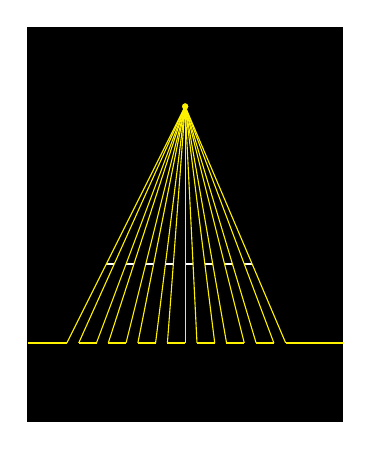
\begin{tikzpicture}
  \coordinate (light) at (0,3);

  \path[use as bounding box] (-2,-1) rectangle (2,4);
  \draw[fill=black] (-2,-1) rectangle (2,4);
  \draw[fill=yellow] (light) circle [radius=0.05cm];
  \draw[yellow,thick,name path=wall] (-2,0) -- (2,0);

  \foreach \x in {-1,-0.75,...,0.75} {
    \draw[white,thick] (\x,1) -- ++(0.1,0);

    \path[name path=ray1] (light) -- ($ (light) ! 5 ! (\x,1) $);
    \path[name path=ray2] (light) -- ($ (light) ! 5 ! (\x + 0.1,1) $);

    \draw[name intersections={of=wall and ray1,by=h1},
          name intersections={of=wall and ray2,by=h2},
          black,thick] (h1) -- (h2);

    \begin{scope}
      \path[clip] (-2,0) rectangle (2,4);
      \draw[yellow,thin] (light) -- ($ (light) ! 5 ! (\x,1) $);
      \draw[yellow,thin] (light) -- ($ (light) ! 5 ! (\x + 0.1,1) $);
    \end{scope}
  }
\end{tikzpicture}

\end{document}